\documentclass[12pt]{article}
\usepackage[english]{babel}
\usepackage[utf8x]{inputenc}
\usepackage{amsmath}
\usepackage{hyperref}
\usepackage[]{algorithm2e}
\usepackage{graphicx}
\usepackage[colorinlistoftodos]{todonotes}


\textheight=250truemm \textwidth=160truemm 
\hoffset=-10truemm \voffset=-20truemm

\begin{document}

\begin{titlepage}

\newcommand{\HRule}{\rule{\linewidth}{0.5mm}} 

\center
 
\textsc{\LARGE Ukrainian Catholic University}\\[1cm]
\textsc{\Large  Faculty of Applied Sciences}\\[0.5cm]
\textsc{\large Business Analytics \& Computer Science Programmes}\\[0.5cm]

\vspace*{1cm}

\HRule \\[0.4cm]
{ \huge \bfseries  Predicting Age by MRI Images Using Regression Based Non-Negative Matrix Factorization }\\[10pt]
{\Large \bfseries Linear Algebra final project report}\\[0.4cm]
\HRule \\[1cm]

\vspace*{1cm}

\Large \emph{Authors:}\\
Volodymyr \textsc{Chernetskyi}\\Olesya \textsc{Tretyak}\\Hermann \textsc{Yavorskyi}\\[1cm]

\vspace*{1cm}
{\large 15 May 2019}\\[2cm]


\includegraphics[height=5cm]{UCU-Apps.png}\\[1cm]

\vfill

\end{titlepage}

\begin{abstract}

	Non-negative matrix factorization is an excellent tool for unsupervised parts-based learning, but proves to be ineffective when parts of a whole follow a specific pattern~\cite{Joshi}. Analyzing such local changes is particularly important when studying anatomical transformations. We implement~\cite{GitHub} an algorithm called Regression based Non-Negative Matrix Factorization (RNMF), which incorporates a regression constraint into the NMF framework, so that it learns maximally changing parts in the basis images.\\ This project is focused on implementing RNMF, rather than implementing NMF or predicting model.

\end{abstract}

\section{Introduction}

	Magnetic Resonance imaging (MRI) is a popular technique used to study the anatomy of the brain. Due to the advancement in technology involved in MRI, the need for automation in related processes has increased. One of such processes is distinguishing brain changes caused by aging between those caused by diseases.

\section{Problem Setting}

	To accurately predict a patient's age by MRI image, we need to extract the most relevant regions of the brain image. We use a matrix decomposition method to simultaneously reduce the dimension of image, thus reducing the number of variables for predictor, and get those relevant regions.
	
	\begin{figure}[h]
		\centering
		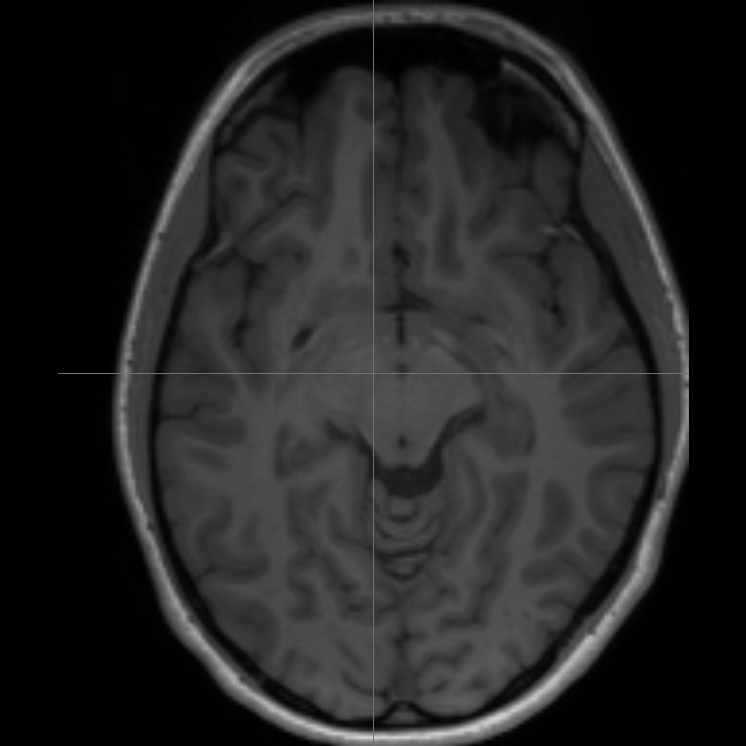
\includegraphics[width=0.5\textwidth]{mri_example.png}
		\caption{\label{fig:example}Example of input MRI image.}
	\end{figure}

	\pagebreak

	There are some well established matrix factorization algorithms in unsupervised learning: Principal Component Analysis (PCA), Independent Component Analysis (ICA) and Non-negative matrix factorization (NMF), that represent data as a linear combination of basis images.\\
	Our solution uses modified NMF to get the work done. NMF ~\cite{Lee}, unlike other matrix factorization algorithms, represents visual information as a sum of its parts - just like people. We combine NMF with regression methods not to only decompose an image into smaller ones, but to choose the most influential ones. 

\section{Solution Description}

	Non-negative matrix factorization (NMF) is distinguished by its use of non-negativity constraints. NMF decomposes a non-negative matrix ($V$) to a set of non-negative bases ($W$) and corresponding non-negative coefficients ($H$),
	$$V_{n*n} \approx W_{n*m}H_{m*n_{t}}$$
	where $V = [v_{i,j}] = [v_{1}, \dots, v_{n_{t}}]$ is a $n*n_{t}$ matrix, where $n$ is the total number of pixels in each image, $v_{j}$ is the \textit{j}th input image represented as a column vector, and $n_{t}$ is the number of images. We denote the basis matrix $W = [w_{i,j}] = [w_{1}, \dots, w_{m}]$ as $n * m$ matrix, $(n + n_{t})m < nn_{t}$. The low dimensional embedding of every column of $V$ is the corresponding column in $H = [h_{i,j}] = [h_{1}, \dots, h_{n_{t}}]$. This factorization is achieved by minimizing the divergence between $V$ and $WH$ applying non-negative constraints. The divergence between $V$ and $Y = WH$ is defined as ~\cite{Lee} ~\cite{Lee2}
	$$D(V||WH) = \sum_{i,j}(v_{ij}\log{\frac{v_{ij}}{y_{ij}} - v_{ij} + y_{ij}})$$
	To implement regression features we should make our data smoothly separated. Which means if labels of $Y$ for corresponding labels of $V$ are close, then corresponding labels in $H$ should reflect this proximity. This is imposed by following constraint:
	$$S_{R} = \frac{\sum_{i,j}f(y_{i}, y_{j})||h_{i} - h_{j}||}{\sum_{i,j}f(y_{i}, y_{j})}$$
	Function $f$ is a heat kernel - weighting function with positive values
	$$f(y_{i}, y_{j}) = \exp(\frac{-||y_{i}-y_{j}||}{t})$$
	$t$ depends on the range of labels. So $f$ will decrease when the distance between data increase. This constraint only considers the labels assigned to each sample in the cross-sectional data. However, if a pair of points have similar labels, but are highly distant in the input space, the influence of such points should be minimized. We compute weights that are inversely proportional to the geodesic distance between the sample points, thus penalizing outliers.
	
	\pagebreak
	
	$$m_{ij} = \frac{d_{ij}}{||v_{i} - v_{j}||}f(y_{i},y_{j})$$
	where $d$ shortest path distance matrix calculated using Floyd's algorithm ~\cite{Cormen} on the graph.Including this in the constraint above we get
	$$S_{Rm} = \frac{\sum_{i,j}m_{ij}||h_{i} - h_{j}||}{\sum_{i,j}m_{ij}}$$
	To outline most regressing features, we are localizing the bases. We are computing bases images $W_{j}$ that are less noisy and restricted to the inclusion of compact regions. Also, local parts should be captured as contiguous regions. To achieve this we minimize the energy of the gradient of each of the basis $W_{j}$ in the image coordinates.
	$$S_{G} = \sum_{j}\int|\nabla W_{j}(x)|^{2}dx$$
	And finally, to minimize the number of basis components required to represent $V$ and to make bases as orthogonal as possible to reduce redundancy between them we minimize ~\cite{Li}
	$$S_O = \sum_{i,j}W^{T}W$$
	The inclusion of the above three constraints leads to the following constrained divergence to be minimized: 
	$$D(V||WH) = \sum_{i,j}(v_{ij}\log{\frac{v_{ij}}{y_{ij}} - v_{ij} + y_{ij}}) + \alpha S_{Rm} + \beta S_{G} + \gamma S_{O}$$
	where $WH = Y$ and $\alpha, \beta, \gamma > 0$ are constants, which are empirically determined such that we get non-negative updates.\\
	The following update rules can be found by minimization of the above constrained divergence:
	$$h_{kl} \leftarrow \frac{-b + \sqrt{b^{2} + (\frac{\sum_{i}v_{il}w_{ik}h'_{kl}}{\sum_{j}w_{ij}h'_{jl}})(\frac{16\alpha m_{kl}}{\sum_{i,j}m_{ij}})}}{\frac{8\alpha m_{kl}}{\sum_{i,j}m_{ij}}} \text{, where } b = 1 - 4\alpha\frac{\sum_{j}h_{kj}m_{jl}}{\sum_{i,j}m_{ij}}$$
	$$w_{kl} \leftarrow \frac{w_{kl}\frac{\sum_{j}v_{kj}h_{lj}}{\sum_{i}w_{il}h_{lj}}}{\sum_{j}h_{lj} + \beta g_{kl} + \gamma \sum_{j}w_{kj}} \text{, where } g = -\nabla^{2}W$$
	$$w_{kl} \leftarrow \frac{w_{kl}}{\sum_{j}w_{jl}}$$
	The proof of convergence is provided in ~\cite{Joshi}.\\\\
	The output is predicted using the linear regression on the lower dimensional representation ($H$).

\section{Implementation}

	NMF algorithm taken from scikit-learn module decomposition.\\
	Linear regression algorithm taken from scikit-learn module linear\_model.\\
	RNMF implemented using numpy.\\

	\begin{algorithm}[H]
		get $V$\ from known and unknown images\;
		apply NMF to $V$\;
		$Y \leftarrow WH$\;
		calculate divergence\;
		\While{difference between old and new divergences is bigger than fixed value}{
			update $H$\;
			update $H$\;
			$Y \leftarrow WH$\;
			calculate divergence\;
		}
		linear\_regression\_model fit(known part of $H$)\;
		linear\_regression\_model predict(unknown part of $H$)\;\
		\caption{Pseudocode}
	\end{algorithm}

\section{Conclusions}

	Using Regression based Non-negative matrix factorization for decomposing MRI images for further predicting the age of the patient is more effective than using basic Non-negative matrix factorization for the same purposes. Moreover, RNMF is more effective than using linear regression without any preprocessing, which means having only the most significant parts of brain image is more effective than having the whole image itself.

\pagebreak

\begin{thebibliography}{9}
	
	\bibitem{Joshi}
	Swapna Joshi., \emph{Anatomical Parts-Based Regression Using Non-Negative Matrix Factorization}, 2010 IEEE Computer Society Conference on Computer Vision and Pattern Recognition, pp. 2863–2870. 
	
	\bibitem{GitHub} \texttt{https://github.com/chernetskyi/anatomical-regression-using-nmf}
	
	\bibitem{Lee}
	Lee D, Seung H.\emph{Learning the parts of objects by nonnegative matrix factorization}, 1999
	
	\bibitem{Lee2}
	Lee D, Seung H.\emph{Algorithms for non-negative matrix factorization. Advances in neural information processing systems}, 2001
	
	\bibitem{Cormen}
	Cormen T, Leiserson C, Rivest R, Stein C. \emph{Introduction to algorithms}, 2001
	
	\bibitem{Li}
	Li S, Hou X, Zhang H, Cheng Q. \emph{Learning spatially localized, parts-based representation}, 2001.
	
\end{thebibliography}

\end{document}